\documentclass[11pt,a4paper]{article}
\usepackage[margin=2.2cm]{geometry}
\usepackage{amsmath,amssymb,bm}
\usepackage{booktabs,array}
\usepackage{enumitem}
\usepackage{xcolor}
\usepackage[breakable,skins]{tcolorbox}
\usepackage{tikz}
\usetikzlibrary{arrows.meta,positioning,calc,fit}
\usepackage{pgfplots}
\pgfplotsset{compat=1.18}
\usepackage[colorlinks=true,linkcolor=blue!50!black,urlcolor=blue!50!black]{hyperref}
\usepackage{fancyhdr}

\definecolor{idea}{RGB}{30,90,160}
\definecolor{exam}{RGB}{20,120,70}
\definecolor{warn}{RGB}{170,60,30}

\newtcolorbox{keyidea}[1][Key idea]{breakable,before upper={\setlength{\parskip}{6pt}},colback=idea!5,colframe=idea!70!black,title={#1},fonttitle=\bfseries}
\newtcolorbox{example}[1][Worked example]{breakable,before upper={\setlength{\parskip}{6pt}},colback=exam!5,colframe=exam!70!black,title={#1},fonttitle=\bfseries}
\newtcolorbox{caution}[1][Watch out]{breakable,before upper={\setlength{\parskip}{6pt}},colback=warn!5,colframe=warn!70!black,title={#1},fonttitle=\bfseries}

\newcommand{\N}{\mathcal{N}}
\newcommand{\Ind}{\mathbb{I}}
\newcommand{\KL}{D_{\mathrm{KL}}}
\newcommand{\Lb}{\mathcal{L}}

\pagestyle{fancy}
\fancyhf{}
\lhead{CSE-5025 Generative AI}
\rhead{Lecture 2 Notes: Classical Latent-Variable Models}
\cfoot{\thepage}
\setlength{\headheight}{14pt}
\setlength{\parindent}{0pt}
\setlength{\parskip}{5pt}

\begin{document}

\begin{center}
{\LARGE\bfseries Lecture 2: Classical Latent-Variable Models}\\[4pt]
{\large Gaussian Mixtures, the EM Algorithm and Hidden Markov Models}\\[6pt]
Study notes with explanations and worked numerical examples\\
CSE-5025 Generative Artificial Intelligence, MS Fall 2026, CSE, University of Dhaka\\
Based on the lecture slides of Dr.\ Mosaddek Hossain Kamal Tushar
\end{center}

\tableofcontents
\newpage

%======================================================================
\section{Recap of Lecture 1 and the Big Picture}
%======================================================================

\subsection{Bayes' rule for latent-variable models}

A \emph{latent-variable generative model} assumes that every observation $x$ is produced by first drawing a hidden (unobserved) variable $z$ and then drawing $x$ given $z$. Bayes' rule links the four quantities we care about:
\[
\underbrace{p_\theta(z\mid x)}_{\text{posterior}}
=\frac{\overbrace{p_\theta(x\mid z)}^{\text{likelihood}}\;\overbrace{p(z)}^{\text{prior}}}{\underbrace{p_\theta(x)}_{\text{evidence}}}.
\]

\begin{itemize}[leftmargin=*]
\item \textbf{Prior $p(z)$}: how probable a latent value is \emph{before} seeing $x$.
\item \textbf{Likelihood $p_\theta(x\mid z)$}: how well a particular $z$ explains the observation. $\theta$ collects all parameters (for a neural network, $\theta=\{W_1,b_1,W_2,b_2,\dots\}$, the weights and biases).
\item \textbf{Posterior $p_\theta(z\mid x)$}: what we believe about $z$ \emph{after} seeing $x$.
\item \textbf{Evidence (marginal likelihood) $p_\theta(x)$}: the probability of $x$ with $z$ ``summed out'':
\[
\text{discrete } z:\; p_\theta(x)=\sum_z p_\theta(x\mid z)\,p(z),
\qquad
\text{continuous } z:\; p_\theta(x)=\int p_\theta(x\mid z)\,p(z)\,dz .
\]
\end{itemize}

Learning means maximum likelihood over a dataset $\{x_n\}_{n=1}^N$:
\[
\theta^\star=\arg\max_\theta \sum_{n=1}^N \log p_\theta(x_n).
\]

\begin{keyidea}
Latent variables let us build a \emph{rich} distribution $p(x)$ out of \emph{simple} parts. But both learning and inference need the posterior $p_\theta(z\mid x)$. Today we study two models where this posterior can be computed \emph{exactly} (GMMs and HMMs) and the algorithm that exploits it (EM).
\end{keyidea}

\subsection{Which parts are easy and which are hard?}

\begin{center}
\begin{tabular}{@{}lll@{}}
\toprule
Component & Difficulty & Reason\\
\midrule
Prior $p(z)$ & Easy & Chosen by us (e.g.\ Gaussian, categorical)\\
Likelihood $p_\theta(x\mid z)$ & Usually manageable & The decoder/model evaluates it for a given $z$\\
Marginal $p_\theta(x)$ & Hard & Sum/integral over \emph{all} latent values\\
Posterior $p_\theta(z\mid x)$ & Hard & Needs $p_\theta(x)$ in the denominator\\
\bottomrule
\end{tabular}
\end{center}

When $z$ takes only a few discrete values (as in GMMs), the ``hard'' sum is just a short finite sum, so everything becomes exact. That is why GMMs are the perfect warm-up before VAEs.

\subsection{Learning objectives}
After this lecture you should be able to:
\begin{enumerate}[nosep]
\item Write the GMM likelihood and explain why maximising it directly is hard.
\item Derive and run the E-step and M-step of EM for a Gaussian mixture.
\item Show that EM maximises a lower bound and never decreases the likelihood.
\item Define an HMM and state its three classical problems.
\item Run the forward, backward and Viterbi recursions on a small example.
\item Explain Baum--Welch as EM for HMMs.
\end{enumerate}

%======================================================================
\section{Gaussian Mixture Models (GMMs)}
%======================================================================

\subsection{Why study GMMs? (GMM vs.\ VAE)}

Both a GMM and a VAE assume data $x$ is generated through a hidden $z$. The difference is the \emph{type} of latent:
\begin{itemize}[nosep]
\item \textbf{GMM}: $z$ is \emph{discrete}; it picks one of $K$ Gaussian components.
\item \textbf{VAE}: $z$ is a \emph{continuous} vector (any real values). A VAE has two neural networks: an \emph{encoder} that learns an approximate posterior $q(z\mid x)$ and a \emph{decoder} that learns the likelihood $p_\theta(x\mid z)$.
\end{itemize}
The mathematical ideas (posterior, evidence, lower bound) are the same, but in a GMM they can be computed exactly, so we can see them clearly.

\subsection{The Gaussian density}

The univariate Gaussian with mean $\mu$ and variance $\sigma^2$ is
\[
\N(x\mid\mu,\sigma^2)=\frac{1}{\sqrt{2\pi\sigma^2}}\exp\!\left(-\frac{(x-\mu)^2}{2\sigma^2}\right).
\]
In $D$ dimensions with covariance $\Sigma$:
$\N(x\mid\mu,\Sigma)=(2\pi)^{-D/2}|\Sigma|^{-1/2}\exp\!\big(-\tfrac12(x-\mu)^\top\Sigma^{-1}(x-\mu)\big)$.

\begin{example}[Example 2.1: Evaluating a Gaussian density]
Evaluate $\N(1\mid 0,1)$ and $\N(1\mid 4,1)$.
\[
\N(1\mid 0,1)=\frac{1}{\sqrt{2\pi}}e^{-(1-0)^2/2}=0.39894\times e^{-0.5}=0.39894\times0.60653=\mathbf{0.24197}.
\]
\[
\N(1\mid 4,1)=0.39894\times e^{-(1-4)^2/2}=0.39894\times e^{-4.5}=0.39894\times0.011109=\mathbf{0.00443}.
\]
The point $x=1$ is about $55$ times more likely under the Gaussian centred at $0$ than under the one centred at $4$. Note that $0.39894=1/\sqrt{2\pi}$ is the peak height of a unit-variance Gaussian.
\end{example}

\subsection{The mixture density}

A Gaussian mixture is a \emph{single} probability distribution formed as a weighted sum of $K$ Gaussians:
\[
\boxed{\;p(x)=\sum_{k=1}^K \pi_k\,\N(x\mid\mu_k,\Sigma_k),\qquad \pi_k\ge 0,\quad \sum_{k=1}^K\pi_k=1.\;}
\]
\begin{itemize}[nosep]
\item $\pi_k$: \textbf{mixing probability} (weight) of component $k$.
\item $\mu_k,\Sigma_k$ (or $\sigma_k^2$ in 1-D): mean and covariance of component $k$.
\item Parameters: $\theta=\{\pi_k,\mu_k,\Sigma_k\}_{k=1}^K$.
\end{itemize}

The figure reproduces the slide's example with $\pi=(0.3,0.5,0.2)$, $\mu=(-2,1,4)$ (unit variances are assumed here for the drawing). Dashed curves are the \emph{weighted} components $\pi_k\N(x\mid\mu_k,1)$; the solid red curve is their sum.

\begin{center}
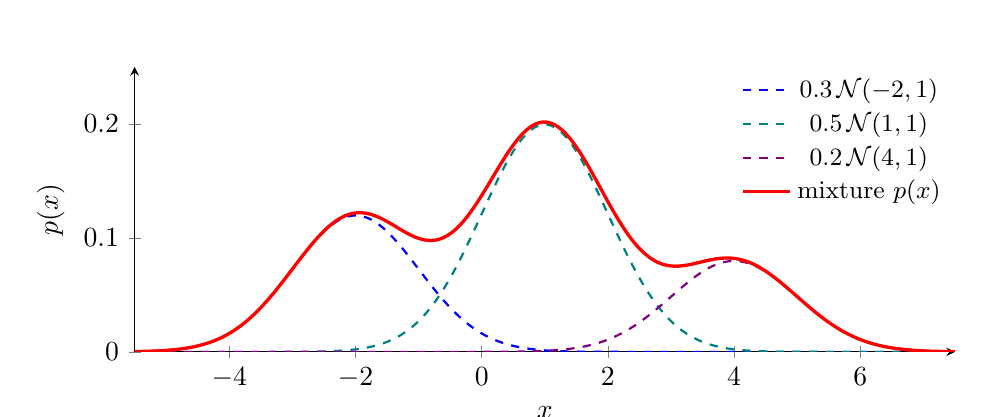
\begin{tikzpicture}
\begin{axis}[width=12cm,height=5.2cm,xmin=-5.5,xmax=7.5,ymin=0,ymax=0.25,
  xlabel={$x$},ylabel={$p(x)$},axis lines=left,samples=200,domain=-5.5:7.5,
  legend style={font=\small,draw=none,at={(1,1)},anchor=north east}]
\addplot[blue,dashed,thick]{0.3*exp(-(x+2)^2/2)/sqrt(2*pi)};
\addplot[teal,dashed,thick]{0.5*exp(-(x-1)^2/2)/sqrt(2*pi)};
\addplot[violet,dashed,thick]{0.2*exp(-(x-4)^2/2)/sqrt(2*pi)};
\addplot[red,very thick]{0.3*exp(-(x+2)^2/2)/sqrt(2*pi)+0.5*exp(-(x-1)^2/2)/sqrt(2*pi)+0.2*exp(-(x-4)^2/2)/sqrt(2*pi)};
\legend{{$0.3\,\N(-2,1)$},{$0.5\,\N(1,1)$},{$0.2\,\N(4,1)$},{mixture $p(x)$}}
\end{axis}
\end{tikzpicture}
\end{center}

\begin{example}[Example 2.2: Evaluating a mixture at a point]
Using the mixture above (unit variances), evaluate $p(x)$ at $x=0$.
\begin{gather*}
\N(0\mid-2,1)=0.39894\,e^{-2}=0.05399,\qquad
\N(0\mid 1,1)=0.39894\,e^{-0.5}=0.24197,\\
\N(0\mid 4,1)=0.39894\,e^{-8}=0.00013.
\end{gather*}
\[
p(0)=0.3(0.05399)+0.5(0.24197)+0.2(0.00013)=0.01620+0.12099+0.00003\approx\mathbf{0.1372}.
\]
Most of the density at $x=0$ comes from the middle component, which is both close and heavily weighted.
\end{example}

\subsection{How a GMM generates data}

\begin{center}
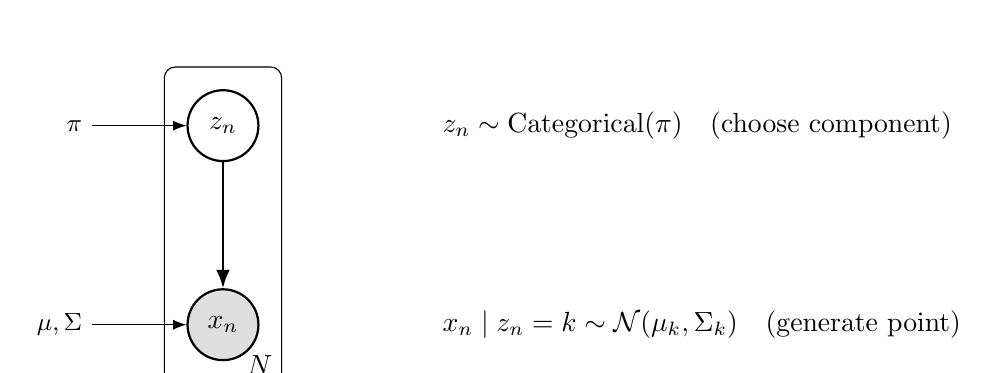
\begin{tikzpicture}[node distance=1.6cm,
  latent/.style={circle,draw,thick,minimum size=9mm},
  obs/.style={circle,draw,thick,fill=gray!25,minimum size=9mm},
  par/.style={font=\small}]
\node[latent] (z) {$z_n$};
\node[obs,below=of z] (x) {$x_n$};
\node[par,left=1.2cm of z] (pi) {$\pi$};
\node[par,left=1.2cm of x] (mu) {$\mu,\Sigma$};
\draw[-{Latex},thick] (z)--(x);
\draw[-{Latex}] (pi)--(z);
\draw[-{Latex}] (mu)--(x);
\node[draw,rounded corners,fit=(z)(x),inner sep=8pt,label={[anchor=south east]south east:$N$}] {};
\node[right=2.2cm of z,align=left] {$z_n\sim\mathrm{Categorical}(\pi)$\quad(choose component)};
\node[right=2.2cm of x,align=left] {$x_n\mid z_n=k\sim\N(\mu_k,\Sigma_k)$\quad(generate point)};
\end{tikzpicture}
\end{center}

Two-step generative process (ancestral sampling):
\begin{enumerate}[nosep]
\item Pick a component: $z_n=k$ with probability $\pi_k$.
\item Draw the observation from that component: $x_n\sim\N(\mu_k,\Sigma_k)$.
\end{enumerate}
The shaded node $x_n$ is observed; $z_n$ is the \emph{discrete latent variable} saying which Gaussian produced $x_n$. The plate ``$N$'' means this repeats independently for each data point.

\begin{example}[Example 2.3: Sampling by hand]
With $\pi=(0.3,0.5,0.2)$, draw a uniform number $u=0.62$. The cumulative weights are $0.3,\;0.8,\;1.0$; since $0.3<0.62\le0.8$, we pick $z=2$. Then draw $x\sim\N(1,1)$, e.g.\ $x=1+1\cdot\epsilon$ with $\epsilon=-0.4$ from a standard normal, giving $x=0.6$. Repeating this many times produces a histogram shaped like the red curve.
\end{example}

\subsection{Joint distribution and marginal likelihood}

\textbf{Joint} (for a specific component $k$): prior times likelihood,
\[
p_\theta(x_n,z_n=k)=\underbrace{p(z_n=k)}_{\pi_k}\;\underbrace{p_\theta(x_n\mid z_n=k)}_{\N(x_n\mid\mu_k,\Sigma_k)}=\pi_k\,\N(x_n\mid\mu_k,\Sigma_k).
\]
\textbf{Marginal}: we never see $z_n$, so we sum it out:
\[
p_\theta(x_n)=\sum_{k=1}^K p_\theta(x_n,z_n=k)=\sum_{k=1}^K\pi_k\,\N(x_n\mid\mu_k,\Sigma_k).
\]
\begin{keyidea}[Important]
Because $z_n$ has only $K$ possible values, marginalisation is a \emph{finite sum}, not an integral. This is exactly what makes the GMM posterior tractable.
\end{keyidea}

\subsection{Why direct maximum likelihood is hard}

For i.i.d.\ data $X=\{x_1,\dots,x_N\}$ the log-likelihood is
\[
\log p(X\mid\theta)=\sum_{n=1}^N\log\Big[\sum_{k=1}^K\pi_k\,\N(x_n\mid\mu_k,\Sigma_k)\Big].
\]
\begin{enumerate}[leftmargin=*]
\item \textbf{Sum inside the log.} Since $\log(a+b)\neq\log a+\log b$, the log cannot ``reach'' the Gaussians to turn them into simple quadratics. Setting the derivative to zero couples all components together and gives no closed-form solution.
\item \textbf{Singularities.} If a mean sits exactly on a data point, $\mu_k=x_1$, then $\N(x_1\mid x_1,\sigma_k^2)=1/\sqrt{2\pi\sigma_k^2}\to\infty$ as $\sigma_k^2\to 0$. The likelihood is unbounded, so the ``maximum'' is a degenerate spike.
\item \textbf{Label switching.} Permuting the component labels gives the same mixture, so there are $K!$ equivalent maxima. (For $K=3$: $3!=6$ identical solutions.)
\end{enumerate}

\begin{example}[Example 2.4: The singularity in numbers]
Take $\mu_1=x_1$. The density of component 1 at $x_1$ is $1/\sqrt{2\pi\sigma_1^2}$:
\[
\sigma_1^2=1\Rightarrow0.399,\qquad \sigma_1^2=0.01\Rightarrow3.99,\qquad \sigma_1^2=10^{-6}\Rightarrow399,\qquad\sigma_1^2\to0\Rightarrow\infty.
\]
The other components keep the remaining points' likelihood finite, so the total log-likelihood goes to $+\infty$. This is a useless solution, which is why in practice we add a small ridge $\epsilon I$ to each covariance (Section~\ref{sec:practice}).
\end{example}

\subsection{What if we knew the labels? (complete data)}

Define the indicator $\Ind[z_n=k]=1$ if $z_n=k$ and $0$ otherwise. If the labels were observed, the \emph{complete-data} log-likelihood would be
\[
\log p(X,Z\mid\theta)=\sum_{n=1}^N\sum_{k=1}^K\Ind[z_n=k]\,\big[\log\pi_k+\log\N(x_n\mid\mu_k,\Sigma_k)\big].
\]
Now the log sits directly on each Gaussian, and the problem splits into $K$ separate easy problems:
\[
N_k=\sum_n\Ind[z_n=k],\qquad \pi_k=\frac{N_k}{N},\qquad \mu_k=\frac{1}{N_k}\sum_{n:z_n=k}x_n,\qquad \Sigma_k=\frac{1}{N_k}\sum_{n:z_n=k}(x_n-\mu_k)(x_n-\mu_k)^\top.
\]
In words: count, average and compute the spread of each group. \textbf{The problem:} in real data the labels $z_n$ are hidden.

\subsection{Responsibilities: soft guesses of the hidden labels}

Although $z_n$ is unknown, Bayes' rule gives its posterior exactly:
\[
\boxed{\;r_{nk}=p(z_n=k\mid x_n,\theta)=\frac{\pi_k\,\N(x_n\mid\mu_k,\Sigma_k)}{\sum_{j=1}^K\pi_j\,\N(x_n\mid\mu_j,\Sigma_j)}\;}
\]
$r_{nk}$ is the \textbf{responsibility} of component $k$ for point $n$. It satisfies $0\le r_{nk}\le1$ and $\sum_k r_{nk}=1$. Instead of a \emph{hard} assignment to one Gaussian, each point is shared \emph{softly} among all components.

\begin{example}[Example 2.5: Responsibilities (from the slides)]
Two components with $\pi_1=0.4$, $\pi_2=0.6$. For a point $x$ the densities are $\N(x\mid\mu_1,\sigma_1^2)=0.8$ and $\N(x\mid\mu_2,\sigma_2^2)=0.2$.

\textbf{Step 1 (numerators $=$ joints):} $\pi_1\N_1=0.4\times0.8=0.32$, \quad $\pi_2\N_2=0.6\times0.2=0.12$.

\textbf{Step 2 (denominator $=$ evidence):} $p(x)=0.32+0.12=0.44$.

\textbf{Step 3 (normalise):}
\[
r_1=\frac{0.32}{0.44}=\mathbf{0.7273},\qquad r_2=\frac{0.12}{0.44}=\mathbf{0.2727},\qquad r_1+r_2=1.
\]
Component 1 takes $72.73\%$ responsibility even though its prior weight ($0.4$) is \emph{smaller}, because it explains $x$ four times better ($0.8$ vs.\ $0.2$). The likelihood outweighs the prior here.
\end{example}

%======================================================================
\section{The EM Algorithm}
%======================================================================

\subsection{The idea in one sentence}

\begin{keyidea}[EM in one sentence]
\textbf{E-step}: use the current parameters to compute the responsibilities (soft labels). \textbf{M-step}: refit each Gaussian as if those soft labels were true, using them as weights. Repeat until the log-likelihood stops improving.
\end{keyidea}

\subsection{EM for Gaussian mixtures: the full algorithm}

\textbf{Initialise} $\theta=\{\pi_k,\mu_k,\Sigma_k\}$ (e.g.\ from $k$-means). Then repeat:

\textbf{E-step} (inference):
\[
r_{nk}=\frac{\pi_k\,\N(x_n\mid\mu_k,\Sigma_k)}{\sum_j\pi_j\,\N(x_n\mid\mu_j,\Sigma_j)}.
\]
\textbf{M-step} (learning; weighted refit):
\[
N_k=\sum_{n=1}^N r_{nk},\qquad
\pi_k=\frac{N_k}{N},\qquad
\mu_k=\frac{1}{N_k}\sum_{n=1}^N r_{nk}\,x_n,\qquad
\Sigma_k=\frac{1}{N_k}\sum_{n=1}^N r_{nk}\,(x_n-\mu_k)(x_n-\mu_k)^\top .
\]
\textbf{Stop} when $\log p(X\mid\theta)$ changes by less than a tolerance.

Compare with the complete-data formulas: EM simply replaces the hard indicator $\Ind[z_n=k]$ with the soft responsibility $r_{nk}$. $N_k$ is the ``effective number of points'' owned by component $k$.

\subsection{Where the M-step formulas come from}

Holding the responsibilities fixed, the M-step maximises the \emph{expected} complete-data log-likelihood
\[
Q(\theta)=\sum_{n=1}^N\sum_{k=1}^K r_{nk}\big[\log\pi_k+\log\N(x_n\mid\mu_k,\Sigma_k)\big].
\]
\textbf{Mean.} Only the Gaussian term depends on $\mu_k$, and $\nabla_{\mu_k}\log\N(x_n\mid\mu_k,\Sigma_k)=\Sigma_k^{-1}(x_n-\mu_k)$. Setting the gradient to zero:
\[
\sum_n r_{nk}\Sigma_k^{-1}(x_n-\mu_k)=0\;\Longrightarrow\;\mu_k\sum_n r_{nk}=\sum_n r_{nk}x_n\;\Longrightarrow\;\mu_k=\frac{1}{N_k}\sum_n r_{nk}x_n.
\]
\textbf{Mixing weights.} We must keep $\sum_k\pi_k=1$, so use a Lagrange multiplier $\lambda$:
\[
\frac{\partial}{\partial\pi_k}\Big[\sum_n\sum_k r_{nk}\log\pi_k+\lambda\big(1-\textstyle\sum_k\pi_k\big)\Big]=\frac{N_k}{\pi_k}-\lambda=0\;\Rightarrow\;\pi_k=\frac{N_k}{\lambda}.
\]
Summing over $k$: $1=\sum_kN_k/\lambda=N/\lambda$, so $\lambda=N$ and $\pi_k=N_k/N$.

\textbf{Covariance.} Differentiating with respect to $\Sigma_k^{-1}$ in the same way gives the weighted sample covariance shown above.

\begin{example}[Example 3.1: One full EM run on a tiny 1-D dataset]
\textbf{Data:} $X=(0,\,1,\,4,\,5)$, $N=4$, $K=2$.\\
\textbf{Initial guess:} $\pi=(0.5,0.5)$, $\mu=(1,4)$, $\sigma^2=(1,1)$.

\medskip
\textbf{Iteration 1, E-step.} For each point compute $\N(x\mid1,1)$, $\N(x\mid4,1)$, multiply by $\pi_k=0.5$ and normalise.
\begin{center}
\begin{tabular}{@{}ccccc@{}}
\toprule
$x_n$ & $\N(x_n\mid1,1)$ & $\N(x_n\mid4,1)$ & $r_{n1}$ & $r_{n2}$\\
\midrule
0 & 0.24197 & 0.00013 & 0.9994 & 0.0006\\
1 & 0.39894 & 0.00443 & 0.9890 & 0.0110\\
4 & 0.00443 & 0.39894 & 0.0110 & 0.9890\\
5 & 0.00013 & 0.24197 & 0.0006 & 0.9994\\
\bottomrule
\end{tabular}
\end{center}
For example, for $x=1$: $r_{11}=\dfrac{0.5(0.39894)}{0.5(0.39894)+0.5(0.00443)}=\dfrac{0.19947}{0.20169}=0.9890$.

\textbf{Iteration 1, M-step.}
\[
N_1=0.9994+0.9890+0.0110+0.0006=2.000,\qquad N_2=2.000,\qquad \pi=(0.5,0.5).
\]
\[
\mu_1=\frac{0.9994(0)+0.9890(1)+0.0110(4)+0.0006(5)}{2.000}=\frac{1.036}{2}=0.518,
\]
\[
\mu_2=4.482\ \text{(by symmetry)}.
\]
\begin{align*}
\sigma_1^2&=\tfrac{1}{2}\big[0.9994(0-0.518)^2+0.9890(1-0.518)^2\\
&\qquad+0.0110(4-0.518)^2+0.0006(5-0.518)^2\big]=0.321,\qquad\sigma_2^2=0.321.
\end{align*}

\textbf{Iteration 2.} With the means pulled into the two clusters and narrower variances, the responsibilities become essentially $1/0$: $\{0,1\}\to$ component 1 and $\{4,5\}\to$ component 2. The M-step then gives
\[
\mu=(0.5,\,4.5),\qquad\sigma^2=(0.25,\,0.25),\qquad \pi=(0.5,0.5),
\]
and further iterations change nothing: EM has \textbf{converged}.

\textbf{Log-likelihood after each iteration.}
\begin{center}
\begin{tabular}{@{}lccc@{}}
\toprule
& Initial & After iter.\ 1 & After iter.\ 2 (converged)\\
\midrule
$\log p(X\mid\theta)$ & $-7.4251$ & $-5.7355$ & $-5.6758$\\
\bottomrule
\end{tabular}
\end{center}
The log-likelihood \emph{rises at every iteration}, as the theory in Section~\ref{sec:whyem} guarantees. The biggest jump comes in the first iteration.
\end{example}

\subsection{\texorpdfstring{$k$}{k}-means as a limiting case of EM}

Fix every covariance to $\Sigma_k=\epsilon I$ and let $\epsilon\to0$. The ratio of two responsibilities for the same point is
\[
\frac{r_{nj}}{r_{nk}}=\frac{\pi_j}{\pi_k}\exp\!\left(-\frac{\|x_n-\mu_j\|^2-\|x_n-\mu_k\|^2}{2\epsilon}\right).
\]
If $\mu_k$ is the nearest centre, the exponent is very negative for every other $j$, so $r_{nj}\to0$. Hence
\[
r_{nk}\to\begin{cases}1 & k=\arg\min_j\|x_n-\mu_j\|^2\\ 0&\text{otherwise.}\end{cases}
\]
\begin{itemize}[nosep]
\item E-step $\to$ \emph{hard} assignment to the nearest centre.
\item M-step $\to$ each centre becomes the mean of its assigned points.
\end{itemize}
That is exactly Lloyd's $k$-means algorithm. Soft EM keeps uncertainty about ambiguous points; $k$-means throws it away. $k$-means is also a good \emph{initialiser} for EM.

\begin{example}[Example 3.2: \texorpdfstring{$k$}{k}-means on the same data]
$X=(0,1,4,5)$, initial centres $(1,4)$. Distances: $0,1$ are closer to $1$; $4,5$ are closer to $4$. New centres: $(0+1)/2=0.5$ and $(4+5)/2=4.5$. The next assignment is unchanged, so $k$-means stops at $(0.5,4.5)$, the same means EM found. The difference is that EM also learns variances and weights and would give fractional responsibilities to a point like $x=2.5$ halfway between the clusters (exactly $0.5/0.5$ here), whereas $k$-means must break the tie arbitrarily.
\end{example}

\subsection{Why EM works: a lower bound on the log-likelihood}\label{sec:whyem}

Take \emph{any} distribution $q(Z)$ over the latent variables. Because $\sum_Z q(Z)=1$ and $p(X\mid\theta)=p(X,Z\mid\theta)/p(Z\mid X,\theta)$:
\begin{align*}
\log p(X\mid\theta)
&=\sum_Z q(Z)\log p(X\mid\theta)
=\sum_Z q(Z)\log\frac{p(X,Z\mid\theta)}{p(Z\mid X,\theta)}\\
&=\sum_Z q(Z)\log\left[\frac{p(X,Z\mid\theta)}{q(Z)}\cdot\frac{q(Z)}{p(Z\mid X,\theta)}\right]\\
&=\underbrace{\sum_Z q(Z)\log\frac{p(X,Z\mid\theta)}{q(Z)}}_{\Lb(q,\theta)\ \text{(lower bound, ELBO)}}
\;+\;\underbrace{\KL\big(q(Z)\,\|\,p(Z\mid X,\theta)\big)}_{\ge0}.
\end{align*}
Since the KL divergence is never negative, $\Lb(q,\theta)\le\log p(X\mid\theta)$ for every $q$. $\Lb$ is the \textbf{evidence lower bound (ELBO)}, the centrepiece of Lecture 3 (VAEs).

\begin{example}[Example 3.3: Checking $\log p=\Lb+\mathrm{KL}$ numerically]
Reuse Example 2.5: the joints are $p(x,z{=}1)=0.32$, $p(x,z{=}2)=0.12$, so $\log p(x)=\ln0.44=-0.8210$ and the true posterior is $r=(0.7273,0.2727)$.

\textbf{A poor guess} $q=(0.5,0.5)$:
\[
\Lb=0.5\ln\frac{0.32}{0.5}+0.5\ln\frac{0.12}{0.5}=0.5(-0.4463)+0.5(-1.4271)=-0.9367,
\]
\[
\KL(q\|r)=0.5\ln\frac{0.5}{0.7273}+0.5\ln\frac{0.5}{0.2727}=0.5(-0.3747)+0.5(0.6061)=0.1157.
\]
$\Lb+\KL=-0.9367+0.1157=-0.8210=\log p(x)$. \checkmark\quad The bound is $0.1157$ below the truth.

\textbf{The best guess} $q=r$ (the E-step choice): $\KL=0$ and
\[
\Lb=0.7273\ln\frac{0.32}{0.7273}+0.2727\ln\frac{0.12}{0.2727}=0.7273\ln0.44+0.2727\ln0.44=\ln0.44=-0.8210.
\]
The bound is now \emph{tight}.
\end{example}

\subsection{EM as coordinate ascent on \texorpdfstring{$\Lb$}{L}}

\begin{center}
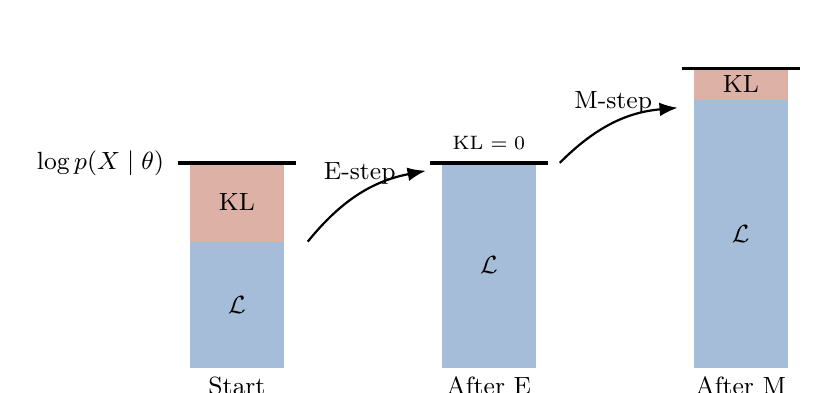
\begin{tikzpicture}[x=1cm,y=1cm]
\foreach \xx/\lab/\Lh/\Ph in {0/Start/1.6/2.6, 3.2/After E/2.6/2.6, 6.4/After M/3.4/3.8}{
  \fill[idea!40] (\xx,0) rectangle ++(1.2,\Lh);
  \fill[warn!40] (\xx,\Lh) rectangle ++(1.2,\Ph-\Lh);
  \draw[very thick] (\xx-0.15,\Ph)--++(1.5,0);
  \node[below] at (\xx+0.6,0) {\small\lab};
}
\node[left] at (-0.2,2.6) {\small$\log p(X\mid\theta)$};
\node at (0.6,0.8) {\small$\Lb$};
\node at (0.6,2.1) {\small KL};
\node at (3.8,1.3) {\small$\Lb$};
\node[font=\scriptsize] at (3.8,2.85) {KL $=0$};
\node at (7.0,1.7) {\small$\Lb$};
\node at (7.0,3.6) {\small KL};
\draw[-{Latex},thick] (1.5,1.6) to[bend left=20] node[above,font=\small]{E-step} (3.0,2.5);
\draw[-{Latex},thick] (4.7,2.6) to[bend left=20] node[above,font=\small]{M-step} (6.2,3.3);
\end{tikzpicture}
\end{center}

\begin{itemize}[leftmargin=*]
\item \textbf{E-step:} set $q(Z)=p(Z\mid X,\theta^{\text{old}})$. Then KL $=0$ and the bound \emph{touches} $\log p$. ($\theta$ does not change, so $\log p$ does not change, but $\Lb$ jumps up to it.)
\item \textbf{M-step:} maximise $\Lb(q,\theta)$ over $\theta$ with $q$ fixed. $\Lb$ rises; and since the new $\theta$ makes the old $q$ no longer the exact posterior, a positive KL reappears, so $\log p$ rises \emph{at least as much} as $\Lb$.
\end{itemize}
\[
\boxed{\;\log p(X\mid\theta^{(t+1)})\;\ge\;\Lb(q^{(t)},\theta^{(t+1)})\;\ge\;\Lb(q^{(t)},\theta^{(t)})\;=\;\log p(X\mid\theta^{(t)})\;}
\]
Read left to right: (bound property) $\ge$ (M-step improved $\Lb$) $\ge$ (E-step made the bound tight). So EM \textbf{never decreases} the log-likelihood. It can, however, converge to a \emph{local} maximum.

\subsection{EM in practice}\label{sec:practice}

\begin{center}
\renewcommand{\arraystretch}{1.25}
\begin{tabular}{@{}p{3.3cm}p{11.7cm}@{}}
\toprule
Issue & Remedy\\
\midrule
Local optima & Several random restarts or $k$-means++ initialisations; keep the run with the best log-likelihood.\\
Collapsing components & Add a small ridge $\epsilon I$ to each $\Sigma_k$, or use a prior on the parameters (MAP-EM).\\
Choosing $K$ & Held-out log-likelihood, or $\mathrm{BIC}=-2\log\hat p+|\theta|\log N$ (smaller is better).\\
Numerical stability & Compute responsibilities in log space with the log-sum-exp trick.\\
Stopping & Relative change in log-likelihood below a tolerance, e.g.\ $10^{-6}$.\\
\bottomrule
\end{tabular}
\end{center}

\begin{example}[Example 3.4: The log-sum-exp trick]
In high dimensions, $\log\pi_k\N(x_n\mid\mu_k,\Sigma_k)$ can be around $-1000$. Then $e^{-1000}$ underflows to $0$ in double precision and $r_{nk}=0/0$. Suppose the two log-joints are $\ell_1=-1000$ and $\ell_2=-1001$. Factor out the maximum $m=-1000$:
\[
\log(e^{\ell_1}+e^{\ell_2})=m+\log\big(e^{\ell_1-m}+e^{\ell_2-m}\big)=-1000+\log(1+e^{-1})=-1000+0.3133=-999.6867.
\]
Then $r_{n1}=e^{\ell_1-(-999.6867)}=e^{-0.3133}=0.7311$ and $r_{n2}=e^{-1.3133}=0.2689$. Nothing underflows.
\end{example}

\begin{example}[Example 3.5: Choosing $K$ with BIC]
For the data $X=(0,1,4,5)$ in 1-D:

\textbf{$K=1$:} the MLE is $\mu=2.5$ and $\sigma^2=\frac14(2.5^2+1.5^2+1.5^2+2.5^2)=4.25$. The squared deviations sum to $17$, so
\[
\log\hat p=-\frac{4}{2}\ln(2\pi\cdot4.25)-\frac{17}{2\cdot4.25}=-6.5696-2=-8.5696.
\]
Parameters: $\mu,\sigma^2$, so $|\theta|=2$ and
\[
\mathrm{BIC}=-2(-8.5696)+2\ln4=17.139+2.773=\mathbf{19.91}.
\]
\textbf{$K=2$:} from Example 3.1, $\log\hat p=-5.6758$. Parameters: one free weight, two means and two variances, so $|\theta|=5$ and
\[
\mathrm{BIC}=-2(-5.6758)+5\ln4=11.352+6.931=\mathbf{18.28}.
\]

$K=2$ has the lower BIC, so it is preferred, even after paying the penalty for 3 extra parameters. (With only 4 points this is just an illustration; real model selection needs much more data.)

In $D$ dimensions with full covariances, $|\theta|=(K-1)+KD+K\,\frac{D(D+1)}{2}$.
\end{example}

%======================================================================
\section{Hidden Markov Models (HMMs)}
%======================================================================

\subsection{From independent points to sequences}

In a GMM every $z_n$ is drawn independently. In many problems the hidden state at time $t$ depends on the state at $t-1$:
phonemes $\to$ audio frames; part-of-speech tags $\to$ words; market regimes $\to$ prices.
An HMM is \emph{a GMM whose component labels form a Markov chain}.

\begin{center}
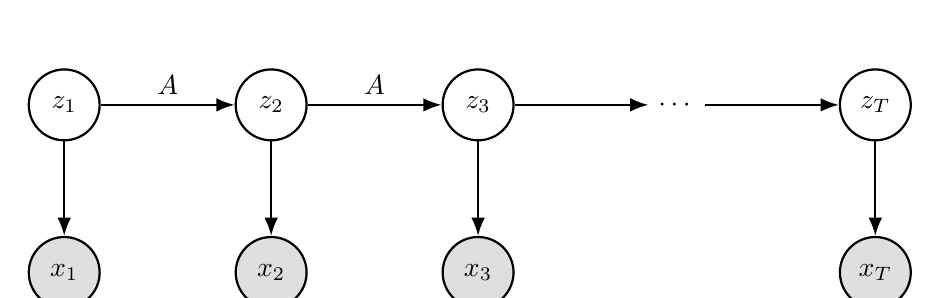
\begin{tikzpicture}[node distance=1.7cm,
  latent/.style={circle,draw,thick,minimum size=9mm},
  obs/.style={circle,draw,thick,fill=gray!25,minimum size=9mm}]
\node[latent] (z1) {$z_1$};
\node[latent,right=of z1] (z2) {$z_2$};
\node[latent,right=of z2] (z3) {$z_3$};
\node[right=of z3] (dots) {$\cdots$};
\node[latent,right=of dots] (zT) {$z_T$};
\foreach \i in {1,2,3,T}{\node[obs,below=1.2cm of z\i] (x\i) {$x_\i$}; \draw[-{Latex},thick] (z\i)--(x\i);}
\draw[-{Latex},thick] (z1)--node[above]{$A$}(z2);
\draw[-{Latex},thick] (z2)--node[above]{$A$}(z3);
\draw[-{Latex},thick] (z3)--(dots);
\draw[-{Latex},thick] (dots)--(zT);
\end{tikzpicture}
\end{center}

The joint distribution factorises as
\[
p(X,Z)=p(z_1)\prod_{t=2}^T p(z_t\mid z_{t-1})\prod_{t=1}^T p(x_t\mid z_t).
\]

\subsection{HMM parameters and assumptions}

\begin{center}
\begin{tabular}{@{}llll@{}}
\toprule
Parameter & Symbol & Definition & Size\\
\midrule
Initial distribution & $\pi$ & $\pi_i=p(z_1=i)$ & $K$\\
Transition matrix & $A$ & $A_{ij}=p(z_t=j\mid z_{t-1}=i)$ & $K\times K$ (rows sum to 1)\\
Emission model & $b_j(x)$ & $p(x_t\mid z_t=j)$ & table or Gaussian per state\\
\bottomrule
\end{tabular}
\end{center}
\textbf{Assumptions:}
\begin{enumerate}[nosep]
\item \emph{First-order Markov}: the next state depends only on the current state.
\item \emph{Output independence}: each observation depends only on its own state.
\end{enumerate}

\begin{example}[Example 4.1: Probability of one specific path]
We use the ice-cream HMM throughout. States: $H$ (hot), $C$ (cold). Observation: ice creams eaten per day, $x\in\{1,2,3\}$.
\[
\pi=(\pi_H,\pi_C)=(0.6,\,0.4),\qquad
A=\begin{pmatrix}A_{HH}&A_{HC}\\A_{CH}&A_{CC}\end{pmatrix}=\begin{pmatrix}0.7&0.3\\0.4&0.6\end{pmatrix},
\]
\begin{center}
\begin{tabular}{@{}cccc@{}}
\toprule
$b_j(x)$ & $x=1$ & $x=2$ & $x=3$\\
\midrule
$H$ & 0.2 & 0.4 & 0.4\\
$C$ & 0.5 & 0.4 & 0.1\\
\bottomrule
\end{tabular}
\end{center}
Observed sequence: $X=(3,1,3)$. The joint probability of the path $Z=(H,H,H)$ is
\[
p(X,Z)=\underbrace{\pi_H b_H(3)}_{0.6\times0.4}\cdot\underbrace{A_{HH}b_H(1)}_{0.7\times0.2}\cdot\underbrace{A_{HH}b_H(3)}_{0.7\times0.4}=0.24\times0.14\times0.28=\mathbf{0.009408}.
\]
To get $p(X)$ we would have to add up such terms for all $2^3=8$ paths. The forward algorithm does this efficiently.
\end{example}

\subsection{The three classical HMM problems}

\begin{center}
\begin{tabular}{@{}llll@{}}
\toprule
Problem & Question & Quantity & Algorithm\\
\midrule
1. Evaluation & How likely is this sequence? & $p(X\mid\theta)$ & Forward\\
2. Decoding & Which hidden path is most likely? & $\arg\max_Z p(Z\mid X)$ & Viterbi\\
3. Learning & Which parameters fit the data? & $\arg\max_\theta p(X\mid\theta)$ & Baum--Welch (EM)\\
\bottomrule
\end{tabular}
\end{center}
Naively each problem ranges over all $K^T$ state sequences. Dynamic programming reduces this to $O(TK^2)$ (Rabiner, 1989).

\begin{example}[Example 4.2: How big is the saving?]
For $K=2$ states and a sequence of length $T=100$: brute force needs $K^T=2^{100}\approx1.27\times10^{30}$ paths, which is hopeless. Dynamic programming needs about $TK^2=100\times4=400$ multiply-adds.
\end{example}

%======================================================================
\section{Inference and Learning in HMMs}
%======================================================================

\subsection{Forward algorithm (evaluation in \texorpdfstring{$O(TK^2)$}{O(TK^2)})}

Define the forward variable as the joint probability of the first $t$ observations \emph{and} being in state $j$ at time $t$:
\[
\alpha_t(j)=p(x_1,\dots,x_t,\;z_t=j).
\]
\begin{align*}
\text{Initialise:}\quad&\alpha_1(j)=\pi_j\,b_j(x_1)\\
\text{Recurse:}\quad&\alpha_t(j)=\Big[\sum_{i=1}^K\alpha_{t-1}(i)\,A_{ij}\Big]\,b_j(x_t)\qquad t=2,\dots,T\\
\text{Terminate:}\quad&p(X)=\sum_{j=1}^K\alpha_T(j)
\end{align*}
\textbf{Why it works:} to be in state $j$ at time $t$ you must have come from \emph{some} state $i$ at $t-1$. $\alpha_{t-1}(i)$ already summarises \emph{all} paths ending in $i$, so we never enumerate paths individually: the $K^T$-term sum is shared.

\begin{example}[Example 5.1: Forward pass for $X=(3,1,3)$]
\textbf{$t=1$, $x_1=3$:}
\[
\alpha_1(H)=\pi_Hb_H(3)=0.6\times0.4=0.2400,\qquad\alpha_1(C)=\pi_Cb_C(3)=0.4\times0.1=0.0400.
\]
\textbf{$t=2$, $x_2=1$:}
\begin{align*}
\alpha_2(H)&=[\alpha_1(H)A_{HH}+\alpha_1(C)A_{CH}]\,b_H(1)=[0.24(0.7)+0.04(0.4)](0.2)=0.0368,\\
\alpha_2(C)&=[\alpha_1(H)A_{HC}+\alpha_1(C)A_{CC}]\,b_C(1)=[0.24(0.3)+0.04(0.6)](0.5)=0.0480.
\end{align*}
\textbf{$t=3$, $x_3=3$:}
\begin{align*}
\alpha_3(H)&=[0.0368(0.7)+0.048(0.4)](0.4)=[0.02576+0.01920](0.4)=0.017984,\\
\alpha_3(C)&=[0.0368(0.3)+0.048(0.6)](0.1)=[0.01104+0.02880](0.1)=0.003984.
\end{align*}
\textbf{Terminate:}
\[
p(X)=\alpha_3(H)+\alpha_3(C)=0.017984+0.003984=\mathbf{0.021968}.
\]
Check: the single best path $(H,H,H)$ from Example 4.1 has probability $0.009408$, about $43\%$ of the total. The other 7 paths make up the rest.
\end{example}

\subsection{Backward pass and state posteriors}

Define the backward variable as the probability of the \emph{future} observations given the current state:
\[
\beta_t(i)=p(x_{t+1},\dots,x_T\mid z_t=i),\qquad\beta_T(i)=1,
\]
\[
\beta_t(i)=\sum_{j=1}^K A_{ij}\,b_j(x_{t+1})\,\beta_{t+1}(j)\qquad t=T-1,\dots,1.
\]
Combining both passes gives the posteriors that learning needs:
\[
\gamma_t(i)=p(z_t=i\mid X)=\frac{\alpha_t(i)\,\beta_t(i)}{p(X)},
\qquad
\xi_t(i,j)=p(z_{t-1}=i,z_t=j\mid X)=\frac{\alpha_{t-1}(i)\,A_{ij}\,b_j(x_t)\,\beta_t(j)}{p(X)}.
\]
$\alpha_t(i)\beta_t(i)=p(X,z_t=i)$: the past and present ($\alpha$) times the future ($\beta$). $\gamma_t(i)$ plays exactly the role of the GMM responsibility $r_{nk}$; $\xi_t(i,j)$ is the posterior probability of using transition $i\to j$ at time $t$.

\begin{example}[Example 5.2: Backward pass and posteriors for $X=(3,1,3)$]
\textbf{Backward, $t=3$:} $\beta_3(H)=\beta_3(C)=1$.

\textbf{$t=2$} (next observation $x_3=3$, so $b_H(3)=0.4$, $b_C(3)=0.1$):
\[
\beta_2(H)=0.7(0.4)(1)+0.3(0.1)(1)=0.31,\qquad \beta_2(C)=0.4(0.4)(1)+0.6(0.1)(1)=0.22.
\]
\textbf{$t=1$} (next observation $x_2=1$, so $b_H(1)=0.2$, $b_C(1)=0.5$):
\[
\beta_1(H)=0.7(0.2)(0.31)+0.3(0.5)(0.22)=0.0434+0.0330=0.0764,
\]
\[
\beta_1(C)=0.4(0.2)(0.31)+0.6(0.5)(0.22)=0.0248+0.0660=0.0908.
\]
\textbf{Sanity check:} $p(X)=\sum_i\pi_ib_i(x_1)\beta_1(i)=0.24(0.0764)+0.04(0.0908)=0.018336+0.003632=0.021968$. \checkmark\ (Same as the forward pass.)

\textbf{State posteriors} $\gamma_t(H)=\alpha_t(H)\beta_t(H)/p(X)$:
\begin{center}
\begin{tabular}{@{}lccc@{}}
\toprule
& $t=1$ & $t=2$ & $t=3$\\
\midrule
$\alpha_t(H)\beta_t(H)$ & $0.24\times0.0764=0.018336$ & $0.0368\times0.31=0.011408$ & $0.017984\times1$\\
$\gamma_t(H)$ & $0.8347$ & $0.5193$ & $0.8186$\\
$\gamma_t(C)=1-\gamma_t(H)$ & $0.1653$ & $0.4807$ & $0.1814$\\
\bottomrule
\end{tabular}
\end{center}
Day 2 (one ice cream) is genuinely uncertain, about $52/48$, but still leans hot because it sits between two hot-looking days.

\textbf{One transition posterior:}
$\xi_2(H,H)=\dfrac{\alpha_1(H)A_{HH}b_H(1)\beta_2(H)}{p(X)}=\dfrac{0.24(0.7)(0.2)(0.31)}{0.021968}=\dfrac{0.010416}{0.021968}=0.4741$.
\end{example}

\subsection{Viterbi algorithm: the most likely state sequence}

Replace the \emph{sum} in the forward recursion with a \emph{max}, and remember which predecessor achieved it:
\begin{align*}
\delta_1(j)&=\pi_j\,b_j(x_1),\\
\delta_t(j)&=\max_i\big[\delta_{t-1}(i)\,A_{ij}\big]\,b_j(x_t),\qquad
\psi_t(j)=\arg\max_i\big[\delta_{t-1}(i)\,A_{ij}\big].
\end{align*}
End at $z_T^\star=\arg\max_j\delta_T(j)$, then backtrack: $z_{t-1}^\star=\psi_t(z_t^\star)$.

$\delta_t(j)$ is the probability of the \emph{best single path} that ends in state $j$ at time $t$. The cost is the same $O(TK^2)$. In practice use log probabilities so that products become sums and nothing underflows.

\begin{example}[Example 5.3: Viterbi for $X=(3,1,3)$]
\textbf{$t=1$:} $\delta_1(H)=0.24$, $\delta_1(C)=0.04$ (same as $\alpha_1$).

\textbf{$t=2$, $x_2=1$:}
\begin{align*}
\delta_2(H)&=\max\{0.24(0.7),\;0.04(0.4)\}\times0.2=\max\{0.168,\;0.016\}\times0.2=0.0336,&\psi_2(H)&=H,\\
\delta_2(C)&=\max\{0.24(0.3),\;0.04(0.6)\}\times0.5=\max\{0.072,\;0.024\}\times0.5=0.0360,&\psi_2(C)&=H.
\end{align*}
\textbf{$t=3$, $x_3=3$:} candidates into $H$: $0.0336(0.7)=0.02352$ (from $H$), $0.036(0.4)=0.01440$ (from $C$); into $C$: $0.0336(0.3)=0.01008$ (from $H$), $0.036(0.6)=0.02160$ (from $C$).
\begin{align*}
\delta_3(H)&=\max\{0.02352,\,0.01440\}(0.4)=0.009408,&\psi_3(H)&=H,\\
\delta_3(C)&=\max\{0.01008,\,0.02160\}(0.1)=0.002160,&\psi_3(C)&=C.
\end{align*}
\textbf{Backtrack:} $z_3^\star=\arg\max\{0.009408,0.002160\}=H$; $z_2^\star=\psi_3(H)=H$; $z_1^\star=\psi_2(H)=H$.

\[
\textbf{Viterbi path: }(H,H,H),\qquad p(X,Z^\star)=0.009408\ \text{(matches Example 4.1)}.
\]

\textbf{Summary table (as on the slides):}
\begin{center}
\begin{tabular}{@{}lccc@{}}
\toprule
& $t=1$ & $t=2$ & $t=3$\\
\midrule
$\alpha_t(H)$ & 0.2400 & 0.0368 & 0.017984\\
$\alpha_t(C)$ & 0.0400 & 0.0480 & 0.003984\\
$\delta_t(H)$ & 0.2400 & 0.0336 & 0.009408\\
$\delta_t(C)$ & 0.0400 & 0.0360 & 0.002160\\
\bottomrule
\end{tabular}
\end{center}
\end{example}

\subsection{The Viterbi trellis and why we backtrack}

\begin{center}
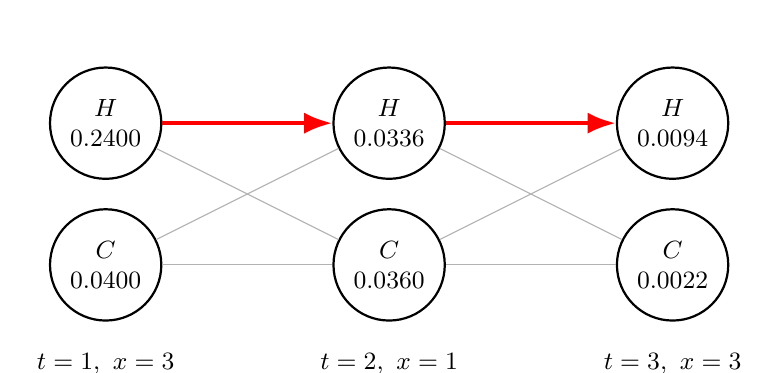
\begin{tikzpicture}[x=3.6cm,y=1.8cm,
  st/.style={circle,draw,thick,minimum size=13mm,align=center,font=\small}]
\foreach \t/\h/\c/\xo in {1/0.2400/0.0400/3, 2/0.0336/0.0360/1, 3/0.0094/0.0022/3}{
  \node[st] (H\t) at (\t,1) {$H$\\\h};
  \node[st] (C\t) at (\t,0) {$C$\\\c};
  \node[font=\small] at (\t,-0.7) {$t=\t,\ x=\xo$};
}
\foreach \a/\b in {1/2,2/3}{
  \draw[gray!60] (H\a)--(C\b); \draw[gray!60] (C\a)--(H\b); \draw[gray!60] (C\a)--(C\b);
}
\draw[red,ultra thick,-{Latex}] (H1)--(H2);
\draw[red,ultra thick,-{Latex}] (H2)--(H3);
\end{tikzpicture}
\end{center}

\begin{caution}[Why not just pick the best state at each time?]
At $t=2$, $\delta_2(C)=0.036>\delta_2(H)=0.0336$, so a greedy choice would say ``cold'' on day 2. Yet the best \emph{whole} path goes through $H$, because a cold day makes three ice creams at $t=3$ unlikely ($b_C(3)=0.1$). The final decision depends on future evidence, so we can only read off the best path by backtracking from the end.
\end{caution}

Note that Viterbi (the best \emph{joint} path) and posterior decoding ($\arg\max_i\gamma_t(i)$ at each $t$ separately) are different questions. Here both give $(H,H,H)$, but in general they can disagree.

\subsection{Baum--Welch: EM for HMMs}

\textbf{E-step:} run the forward and backward passes; compute $\gamma_t(i)$ and $\xi_t(i,j)$.

\textbf{M-step:} re-estimate the parameters from \emph{expected counts}:
\[
\pi_i=\gamma_1(i),\qquad
A_{ij}=\frac{\sum_{t=2}^T\xi_t(i,j)}{\sum_{t=2}^T\sum_{j'}\xi_t(i,j')},\qquad
b_j(v)=\frac{\sum_t\gamma_t(j)\,\Ind[x_t=v]}{\sum_t\gamma_t(j)}.
\]
\begin{itemize}[nosep]
\item $A_{ij}$ = (expected number of $i\to j$ transitions) / (expected number of transitions out of $i$). The denominator equals $\sum_{t=1}^{T-1}\gamma_t(i)$.
\item $b_j(v)$ = (expected times in state $j$ while seeing $v$) / (expected times in state $j$).
\item Expected counts replace observed counts, just like $r_{nk}$ replaced $\Ind[z_n=k]$ in the GMM.
\item \emph{Gaussian emissions}: use the GMM M-step with $\gamma_t(j)$ in place of $r_{nk}$.
\item \emph{Long sequences}: scale $\alpha,\beta$ at each step or work in log space.
\end{itemize}

\begin{example}[Example 5.4: One Baum--Welch update from $X=(3,1,3)$]
Using $\gamma$ from Example 5.2 and all four $\xi$ values at each time:
\begin{center}
\begin{tabular}{@{}lcccc@{}}
\toprule
& $\xi_t(H,H)$ & $\xi_t(H,C)$ & $\xi_t(C,H)$ & $\xi_t(C,C)$\\
\midrule
$t=2$ & 0.4741 & 0.3605 & 0.0452 & 0.1202\\
$t=3$ & 0.4690 & 0.0503 & 0.3496 & 0.1311\\
\bottomrule
\end{tabular}
\end{center}
(Each row sums to 1, as it must.)

\textbf{Initial distribution:} $\pi^{\text{new}}=(\gamma_1(H),\gamma_1(C))=(0.8347,\,0.1653)$.

\textbf{Transition $H\to H$:}
\[
A_{HH}^{\text{new}}=\frac{0.4741+0.4690}{(0.4741+0.3605)+(0.4690+0.0503)}=\frac{0.9431}{1.3539}=0.6966,\qquad A_{HC}^{\text{new}}=0.3034.
\]
\textbf{Emission $b_H(3)$:} $x=3$ occurs at $t=1,3$:
\[
b_H^{\text{new}}(3)=\frac{\gamma_1(H)+\gamma_3(H)}{\gamma_1(H)+\gamma_2(H)+\gamma_3(H)}=\frac{0.8347+0.8186}{0.8347+0.5193+0.8186}=\frac{1.6533}{2.1726}=0.7610.
\]
Similarly $b_H^{\text{new}}(1)=0.5193/2.1726=0.2390$ and $b_H^{\text{new}}(2)=0$.

\textbf{Lesson:} $b_H(2)$ becomes $0$ because ``2'' never appears in this tiny sequence. With real data we train on many long sequences and often add pseudo-counts (smoothing) to avoid zero probabilities.
\end{example}

\subsection{Putting it together: GMM vs.\ HMM}

\begin{center}
\begin{tabular}{@{}lll@{}}
\toprule
& GMM & HMM\\
\midrule
Latent structure & Independent $z_n$ & Markov chain $z_1\to\cdots\to z_T$\\
Posterior quantity & $r_{nk}$ & $\gamma_t(i)$, $\xi_t(i,j)$\\
E-step cost & $O(NK)$ & $O(TK^2)$ via forward--backward\\
Learning & EM & Baum--Welch (EM)\\
Exact posterior? & Yes & Yes\\
\bottomrule
\end{tabular}
\end{center}

\begin{keyidea}[Looking ahead to Lecture 3]
Both models work because the latent space is \emph{small and discrete}, so the E-step can compute $p(Z\mid X,\theta)$ exactly. With a \emph{continuous, high-dimensional} $z$ and a neural-network decoder, the exact E-step is impossible. We then pick $q$ from a tractable family and maximise the ELBO $\Lb(q,\theta)$ directly: this is variational inference, and it leads to the VAE.
\end{keyidea}

%======================================================================
\section{In-Class Exercise: Worked Solutions}
%======================================================================

\begin{example}[Exercise 1: GMM responsibilities]
1-D GMM, $K=2$, $\pi=(0.5,0.5)$, $\mu=(0,4)$, $\sigma^2=(1,1)$. Find $r_{n1}$ for $x_n=1$ and $x_n=2$.

Equal weights and equal variances mean that $\pi_k$ and $1/\sqrt{2\pi}$ cancel:
\[
r_{n1}=\frac{e^{-(x_n-0)^2/2}}{e^{-(x_n-0)^2/2}+e^{-(x_n-4)^2/2}}.
\]
\textbf{$x_n=1$:}
$r_{n1}=\dfrac{e^{-0.5}}{e^{-0.5}+e^{-4.5}}=\dfrac{1}{1+e^{-4}}=\dfrac{1}{1+0.01832}=\mathbf{0.9820}$.
(Using Example 2.1: $0.24197/(0.24197+0.00443)=0.9820$.)

\textbf{$x_n=2$:} the point is equally far from $0$ and $4$, so
$r_{n1}=\dfrac{e^{-2}}{e^{-2}+e^{-2}}=\mathbf{0.5}$.
\end{example}

\begin{example}[Exercise 2: Forward variables in the ice-cream HMM for $X=(1,1)$]
\textbf{$t=1$, $x_1=1$:} $\alpha_1(H)=0.6\times0.2=0.12$, \quad $\alpha_1(C)=0.4\times0.5=0.20$.

\textbf{$t=2$, $x_2=1$:}
\begin{align*}
\alpha_2(H)&=[0.12(0.7)+0.20(0.4)]\times0.2=[0.084+0.080]\times0.2=\mathbf{0.0328},\\
\alpha_2(C)&=[0.12(0.3)+0.20(0.6)]\times0.5=[0.036+0.120]\times0.5=\mathbf{0.0780}.
\end{align*}
So $p(X)=0.0328+0.0780=0.1108$, and two days of one ice cream point towards cold weather.
\end{example}

\begin{example}[Exercise 3: Why EM never decreases the log-likelihood]
The E-step makes the lower bound $\Lb$ equal to $\log p$ (KL $=0$), and the M-step can only raise $\Lb$, which is always below $\log p$, so the new $\log p$ is at least the old one.
\end{example}

%======================================================================
\section{Summary and Formula Sheet}
%======================================================================

\begin{itemize}[leftmargin=*]
\item \textbf{GMM:} $p(x)=\sum_k\pi_k\N(x\mid\mu_k,\Sigma_k)$. Direct MLE is hard because the sum sits inside the log; the likelihood also has singularities and $K!$ label symmetries.
\item \textbf{Responsibilities:} $r_{nk}=\pi_k\N_k/\sum_j\pi_j\N_j$, i.e.\ Bayes' rule on the hidden label.
\item \textbf{EM for GMM:} E: compute $r_{nk}$. M: $N_k=\sum_nr_{nk}$, $\pi_k=N_k/N$, $\mu_k=\frac1{N_k}\sum_nr_{nk}x_n$, $\Sigma_k=\frac1{N_k}\sum_nr_{nk}(x_n-\mu_k)(x_n-\mu_k)^\top$.
\item \textbf{$k$-means} is EM with $\Sigma_k=\epsilon I$, $\epsilon\to0$ (hard assignments).
\item \textbf{ELBO:} $\log p(X\mid\theta)=\Lb(q,\theta)+\KL(q\|p(Z\mid X,\theta))$. EM is coordinate ascent on $\Lb$ and never decreases the likelihood.
\item \textbf{HMM:} $p(X,Z)=\pi_{z_1}\prod_tA_{z_{t-1}z_t}\prod_tb_{z_t}(x_t)$.
\item \textbf{Forward:} $\alpha_t(j)=[\sum_i\alpha_{t-1}(i)A_{ij}]b_j(x_t)$, $p(X)=\sum_j\alpha_T(j)$.
\item \textbf{Backward:} $\beta_t(i)=\sum_jA_{ij}b_j(x_{t+1})\beta_{t+1}(j)$, $\beta_T=1$.
\item \textbf{Posteriors:} $\gamma_t(i)=\alpha_t(i)\beta_t(i)/p(X)$; $\xi_t(i,j)=\alpha_{t-1}(i)A_{ij}b_j(x_t)\beta_t(j)/p(X)$.
\item \textbf{Viterbi:} $\delta_t(j)=\max_i[\delta_{t-1}(i)A_{ij}]b_j(x_t)$, store $\psi_t(j)$, backtrack.
\item \textbf{Baum--Welch:} EM for HMMs with expected state and transition counts.
\item All HMM recursions cost $O(TK^2)$ instead of $O(K^T)$.
\item Exact E-steps need small discrete latents; beyond that we need variational inference (Lecture 3).
\end{itemize}

\subsection*{Before next time}
\textbf{Reading:} Rabiner (1989), ``A Tutorial on Hidden Markov Models and Selected Applications in Speech Recognition,'' \emph{Proc.\ IEEE}; Blei et al.\ (2017), ``Variational Inference: A Review for Statisticians,'' \emph{JASA}, Sections 1--2.

\textbf{Assignment A1 (due Lecture 4):} implement EM for a GMM from scratch and plot the log-likelihood per iteration; implement forward and Viterbi for a discrete HMM and verify against the ice-cream example (Examples 5.1 and 5.3 give every intermediate number to check against).

\end{document}
